\documentclass{article}
\usepackage[margin=0.25in]{geometry}
\usepackage{blindtext}
\usepackage{pgfplots}
\pgfplotsset{width=10cm,compat=1.9}
\usetikzlibrary{automata,positioning}

% We will externalize the figures
\usepgfplotslibrary{external}
%\tikzexternalize

\begin{document}
	
	\tableofcontents
	
	\pagenumbering{gobble}% Remove page numbers (and reset to 1)
	\clearpage
	\section{Graphs}
	\pagestyle{plain}
	\pagenumbering{arabic}% Capital 'R': uppercase Roman numerals
	
	First example is 2D and 3D math expressions plotted side-by-side.
	
	\vskip 10pt
	
	%Here begins first 2D plot
	\begin{tikzpicture}
		\begin{axis}
			\addplot[color=red]{exp(x)};
			\addplot[color=green]{50};
		\end{axis}
	\end{tikzpicture}
	%Here ends first 2D plot
	
	\vskip 10pt
	
	%Here begins first 3D plot
	\begin{center}
		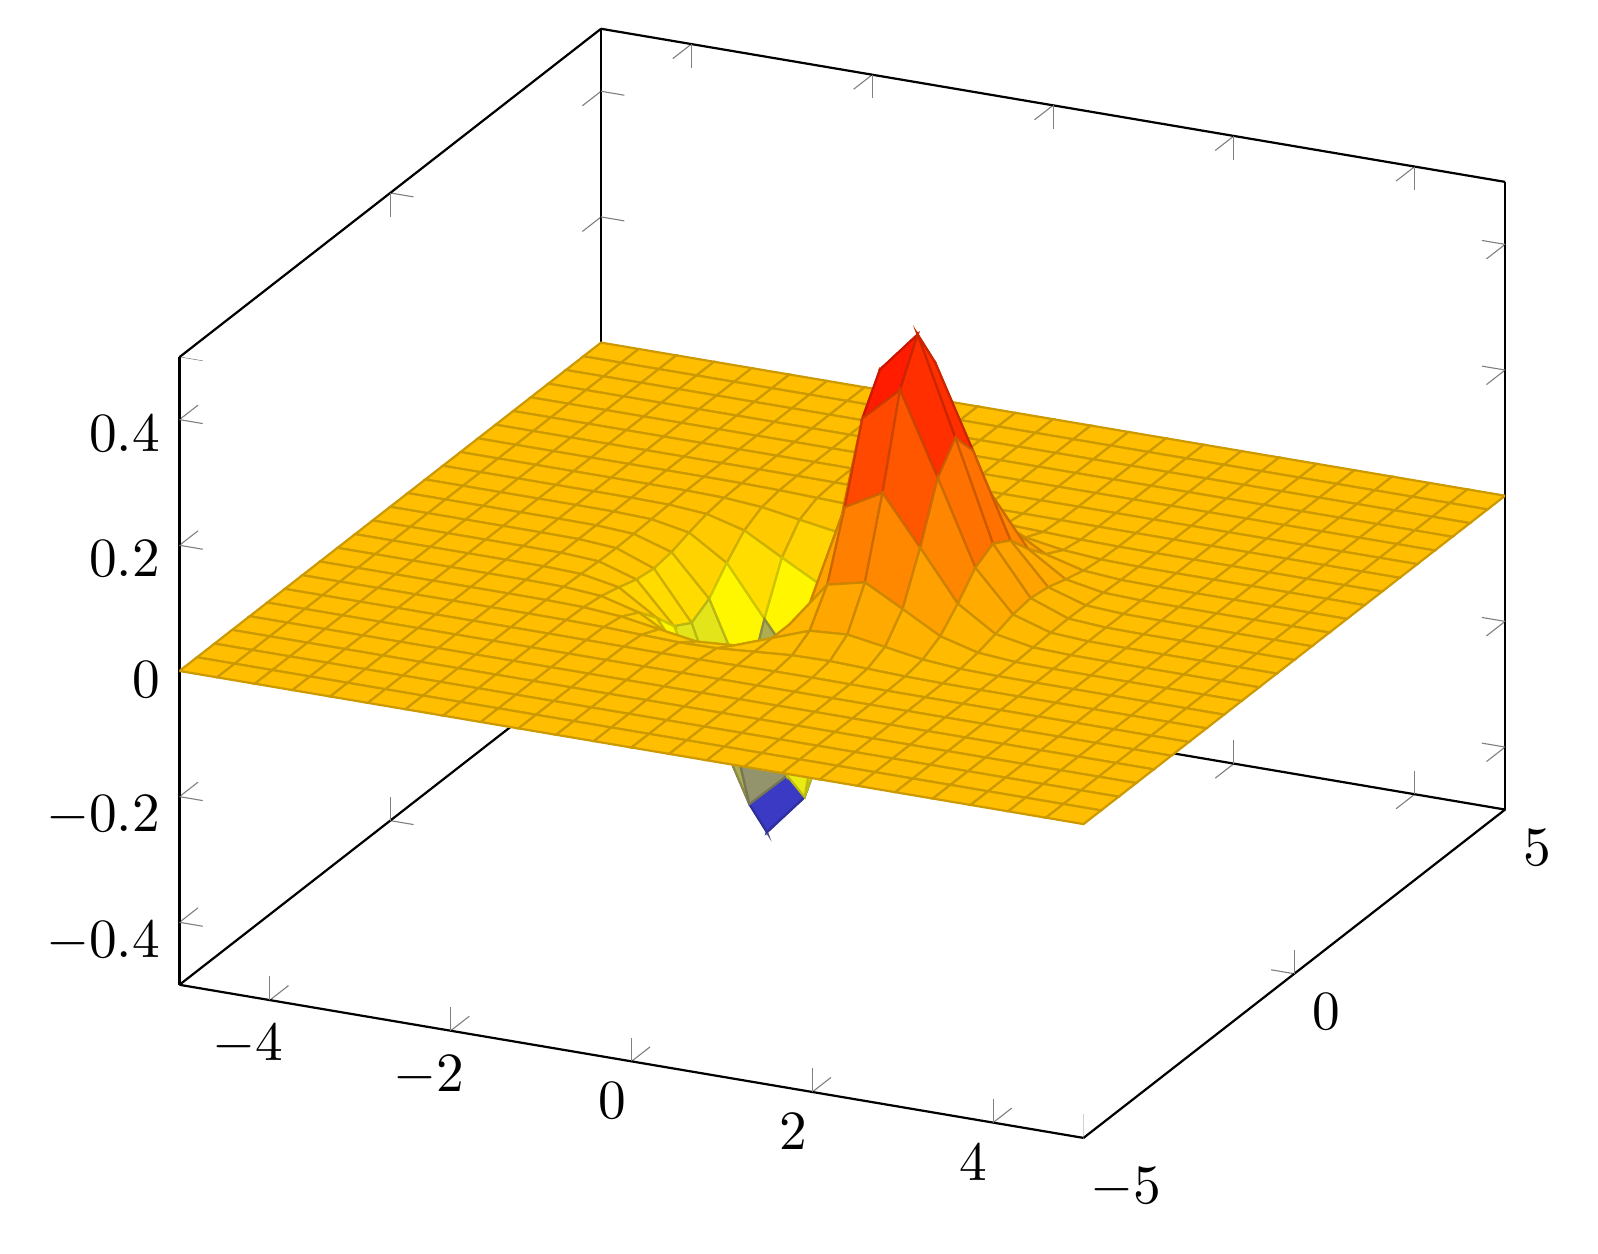
\begin{tikzpicture}[scale = 2]
			\begin{axis}
				%surf - surface plot
				\addplot3[surf,]{exp(-x^2-y^2)*x};
			\end{axis}
		\end{tikzpicture}
	\end{center}
	%Here ends first 3D plot
	
	\vskip 10pt
	
	%Here begins second 2D plot
	\begin{tikzpicture}
		\begin{axis}[
			%Axis configuration
			axis lines = left,
			xlabel = \(x\),
			ylabel = {\(f(x)\)}, 
			legend cell align={left}, % The command for legend alignment
			legend pos = south east
			]
			
			%Red parabola is defined
			\addplot[
				domain= -10:10,
				samples = 100,
				color = red,
				]
				{x^2 - 2*x -1};
			\addlegendentry{\(x^2 - 2x -1\)}
			
			%Blue parabola is defined
			\addplot[
				domain= -10:15,
				samples=100,
				color=blue,
				]
				{x^2 + 2*x +1};
			\addlegendentry{\(x^2 + 2x +1\)};
			
			%Black curve is defined
			\addplot[
				domain= -10:10,
				samples = 100,
				color = black,
				]
				{x^3 - 3*x -1};
			\addlegendentry{\(test\)};
		\end{axis}
	\end{tikzpicture}

	\clearpage
	
	Plotting from data:
	\begin{figure}[h]
		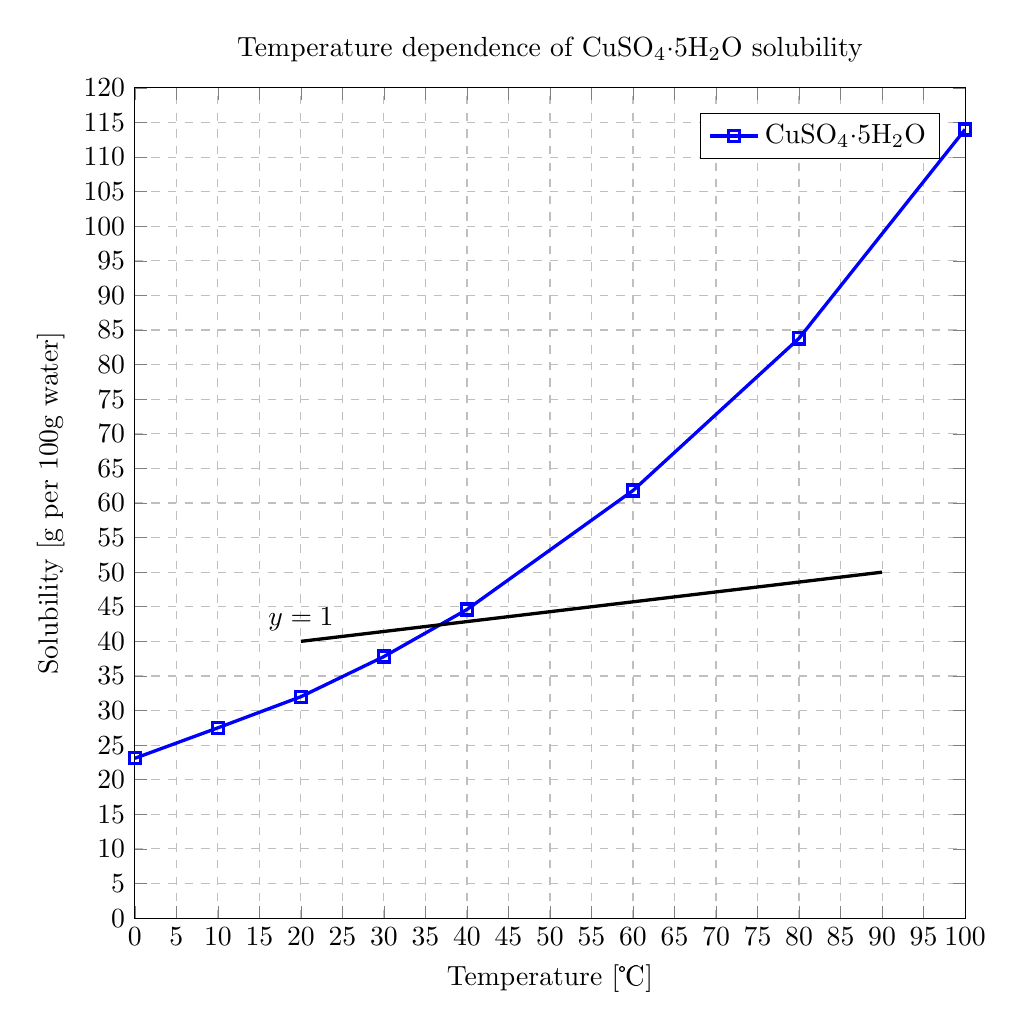
\begin{tikzpicture}
			\begin{axis}[
				title={Temperature dependence of CuSO\(_4\cdot\)5H\(_2\)O solubility},
				xlabel={Temperature [\textcelsius]},
				ylabel={Solubility [g per 100g water]},
				width = \textwidth,
%				height = \textwidth/2,
				height = \textwidth,
				xmin=0, xmax=100,
				ymin=0, ymax=120,
%				xtick={0,20,40,60,80,100},
				xtick={0, 5,...,100},
%				ytick={0,20,40,80,100,120},
				ytick={0, 5,...,120},
				legend pos = north east,
				ymajorgrids = true,
				xmajorgrids = true,
				grid style = dashed,
				yticklabel style={/pgf/number format/precision=2}, 
				xticklabel style={/pgf/number format/precision=3},
				]
		
				\addplot[
%					domain = -10:110,
					color = blue,
					very thick,
					mark = cube
					]
					coordinates {		(0,23.1)(10,27.5)(20,32)(30,37.8)(40,44.6)(60,61.8)(80,83.8)(100,114)
					};
					\legend{CuSO\(_4\cdot\)5H\(_2\)O}
				\draw[
					very thick,
					.-.
					]
					(20,40) node[above] {$y = 1$} -- (90, 50);
			\end{axis}
		\end{tikzpicture}
	\end{figure}

	\vskip 10pt
	
	\clearpage
	
	Bar graph:
	
	\vskip 10pt
	
	\begin{figure}[h]
		\begin{center}
			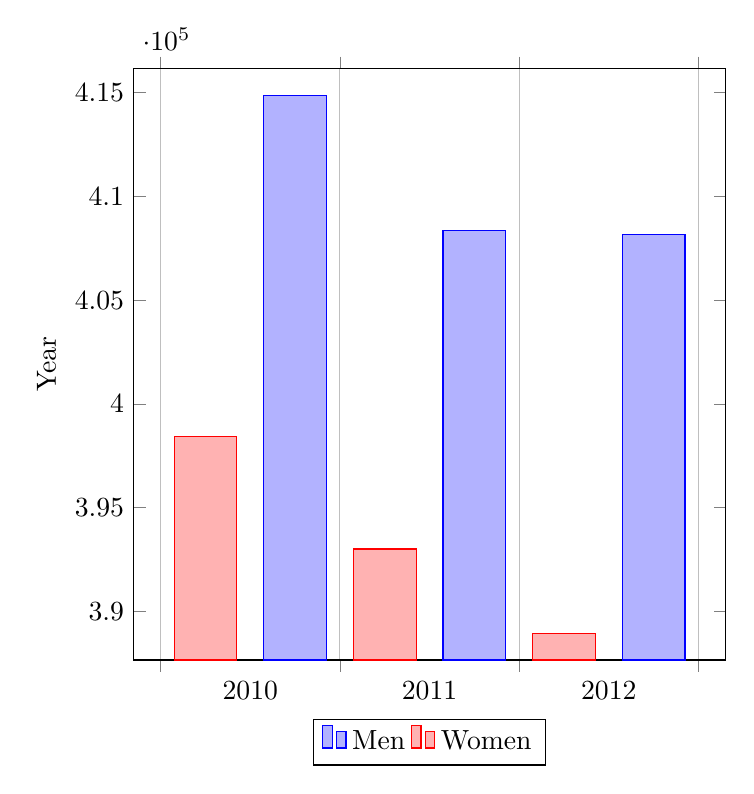
\begin{tikzpicture}
				\begin{axis}[
						width = .75\textwidth,
						height = .75\textwidth,
						x tick label style = {/pgf/number format/1000 sep=},
						ylabel = Year,
						enlargelimits = 0.05,
						legend style = {at = {(0.5, -0.1)}, anchor = north, legend columns = -1},
						ybar interval = 0.7
						]
						
					\addplot 
						coordinates {(2012,408184) (2011,408348) (2010,414870) (2009,412156)};
					\addplot 
						coordinates {(2012,388950) (2011,393007) (2010,398449) (2009,395972)};
					\legend{Men, Women}
				\end{axis}
			\end{tikzpicture}
		\end{center}
	\end{figure}

	\vskip 10pt
	
	\clearpage
	
	Plotting a surface from data:
	
	\vskip 10pt
	
	\begin{figure}[h]
		\begin{center}
			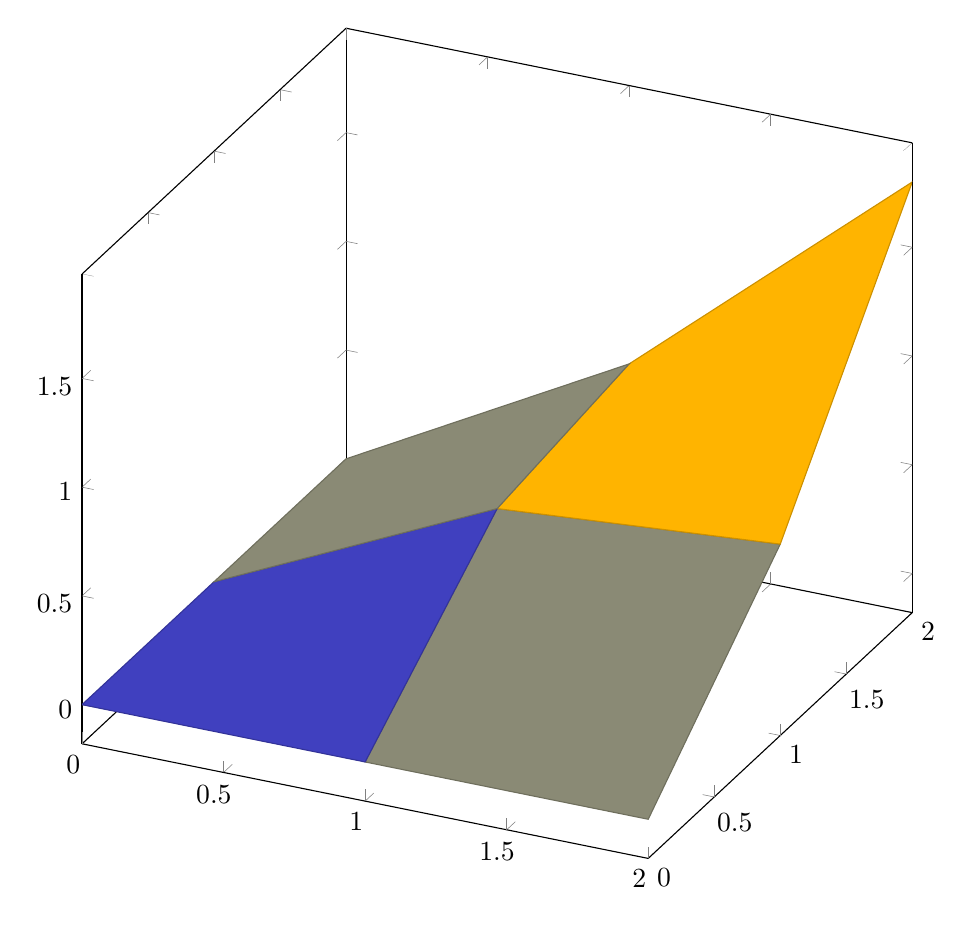
\begin{tikzpicture}
				\begin{axis}[
					width = \textwidth,
					%				height = \textwidth/2,
					height = \textwidth,
					]
					\addplot3[
						surf,
						]
					coordinates {
						(0,0,0) (0,1,0) (0,2,0)
						
						(1,0,0) (1,1,0.6) (1,2,0.7)
						
						(2,0,0) (2,1,0.7) (2,2,1.8)
					};
				\end{axis}
			\end{tikzpicture}
		\end{center}
	\end{figure}
	
	\clearpage
	
	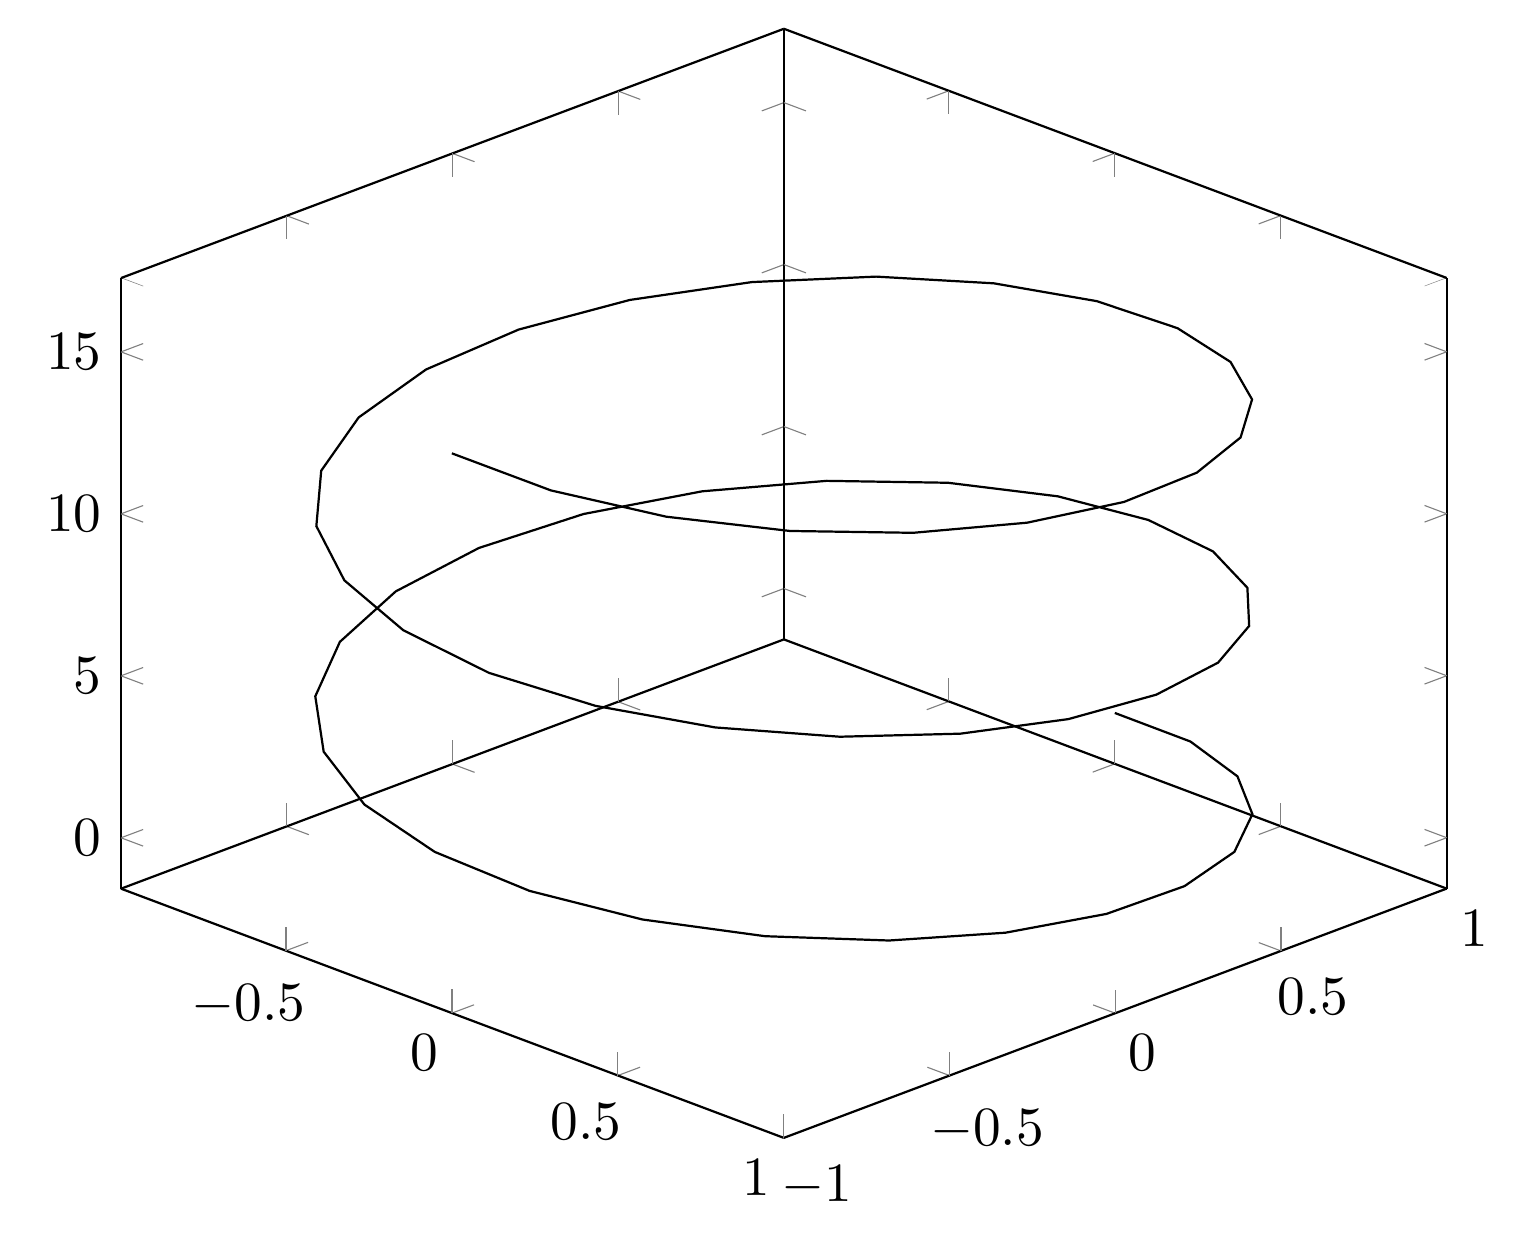
\begin{tikzpicture}[scale = 2]
		\begin{axis}
			[
			view={45}{30},
			]
			\addplot3[
			domain=0:5*pi,
			samples = 60,
			samples y=0,
			]
			({sin(deg(x))},
			{cos(deg(x))},
			{x});
		\end{axis}
	\end{tikzpicture}
	
	\vskip 10pt
	
	\blindtext

	
\end{document}